\documentclass{article}
\usepackage[utf8]{inputenc}
\usepackage{fancyhdr}
\pagestyle{fancy}
\usepackage{natbib}
\usepackage{graphicx}
\usepackage{textcomp}
\usepackage{array}
\usepackage{tabulary}
\newcolumntype{K}[1]{>{\centering\arraybackslash}p{#1}}


% Define the headers and footers for the document
\lhead{Malcolm Watt}
\lfoot{}
\cfoot{\thepage}
\rfoot{}

% Title authors and date

\title{\Huge{Enigma}}
\author{
    Watt, Malcolm \\
    260585950
}
\date{April 15, 2016}


 % ---------- Start of the document ------------
 % Needs Review
 %A header listing the group number and the names and student numbers of each group member. 

 % Needs Review
 %• A title, giving the name of your system. 

 % Needs Review
 %• A description of the system's features (like an advertising brochure describing what the system does). 

 % Needs Review
 %• A block diagram of the entire system. 
 %• A detailed description of how your system works, referring to the block diagram. 

 % Needs Review
 %• A description of the user interface (i.e. a users guide to operation). 

 % 
 %• A discussion of how the complete system was tested. 

 %• A summary of the FPGA resource utilization and timing. 

 % 
 %• A conclusion section discussing problems or significant issues that arose during the design process, as well as a discussion of possible enhancements or extensions that could be made to your system.
 % The ability to rotate the rotors back by one if you make a mistake so that you don't have to restart the entire transmission of your message
 % The ability to see how many characters you have supposedly encrypted, this way you can see where you are in your word, which helps with the previous enhancement ^^
 % With a more sophisticated LED display, you could effectively write whole words out and encrypt them in one shot. This would reduce errors, and make the process easier
 % Have an actual keyboard, with a letter for each of the keys
 % include a few synthax characters, (space, comma, period)
 
\begin{document}

\maketitle

\section{Features}
A sophisticated and easy to use encryption system. Allows easy encryption of messages which can be decoded at any time by an individual with access to your initial settings. There are millions of possible starting configurations, so unscrambling your messages will be practically impossible for unintended third parties. 

The intuitive setup mode allows you to set a variety of options, from the type of reflector to use, to the initial position of the rotors of your machine. All of which impact encryption and make your messages more secure. 

The user interface allows you to see which letter you are attempting to encrypt, and with the click of a button you can encrypt it and see the output and the input side by side. The converted output remains valid until you click the button again, meaning you do not have to hold the button down to read the encrypted letter, freeing your hands up to work more effectively. 

Made a mistake and need to go back to your starting rotor positions? This is accomplished by the simple click of a button thanks to the well organized Enigma setup tools.

\clearpage

\tableofcontents

\clearpage

\section{System Description}
This section is a technical description of the Enigma machine. We're going to take a top down approach to the system and its components, starting at the highest level and working our way down. Naturally let us then start with an explanation of the system's high level inputs and outputs. Figure \ref{fig:full_sys_block_diag} shows the block diagram of the overall system. This system toggles between operation mode and setup mode based on the \textit{setup\_switch}. When in operation mode, the input is determined based on the five slide switches that make up \textit{input\_code}, and the letter is encoded by hitting the button routed to \textit{value\_key}. A detailed description of how to operate the machine is discussed in section \ref{oppmode}, while a detailed explanation of how to set up the Enigma is discussed in section \ref{config}. 

Now we will go one step deeper and look at the contents of the Enigma user interface. 

\begin{figure}[ht!]
    \centering
    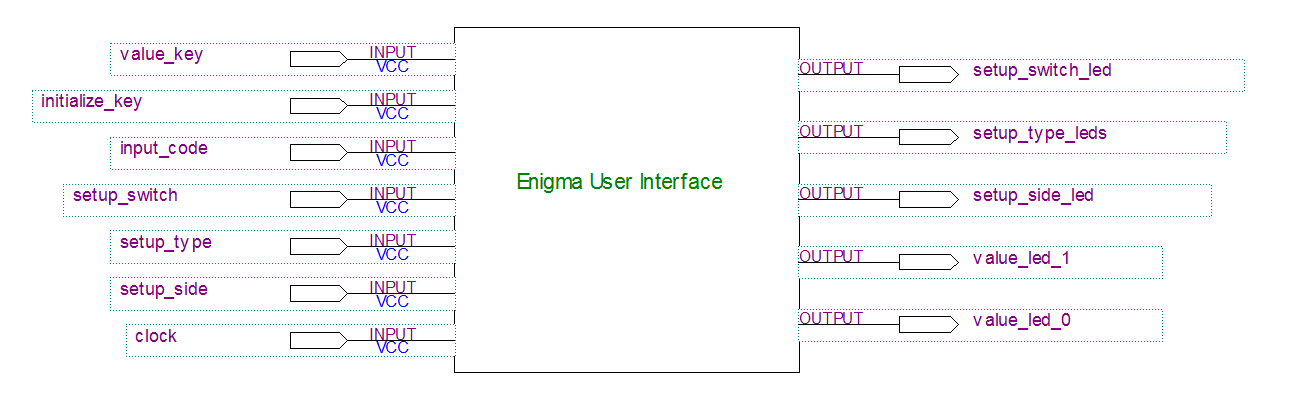
\includegraphics[scale=0.3]{full_sys_block_diag.PNG}
    \caption{The top level block diagram of the Enigma user interface.}
    \label{fig:full_sys_block_diag}
\end{figure}

\subsection{Interface Implementation}
Once you have a chance to see how the different setup modes are toggled between in section \ref{switches}, it will become clear that the different operation modes are being chosen based on a multiplexed system where the setup inputs choose between a set of configuration modes on the machine. Knowing this it will not be surprising to see that this is exactly how Quartus interprets the underlying VHDL. In figure \ref{fig:ui_block_diagram} we can see the general layout of the user interface, however, there is a lot going on and the details are difficult to interpret. Generally you see the multiple layers of multiplexers that make up the selection of modes and settings, along with a set of D-flip-flops to retain the settings once they have been set. The specifics of this part are not particularly interesting, as they are simply the CAD tools rendering of a set of VHDL \textbf{case} statements. 

In order to see closer let's examine figures \ref{fig:seven_segment_decoders} and \ref{fig:enig_block_diag}. Here we can see the next layer of depth in both the way that we decode the outputs from 5 bit numbers into letter representations for the 7 segment LEDs, as well as the actual underlying Enigma machine. The Enigma machine's block diagram in figure \ref{fig:enig_block_diag} shows all of the inputs and outputs of the scrambling mechanism. The seven segment decoder's functionality is trivial, in that it converts a 5 bit number between 0 and 25 into its corresponding letter of the alphabet and asserts the corresponding signals for the seven segment display. There is no use discussing the internal workings of this any further and instead, in the following sections, we will discuss the implementation of the scrambling mechanisms within the Enigma. 

\begin{figure}[ht!]
    \centering
    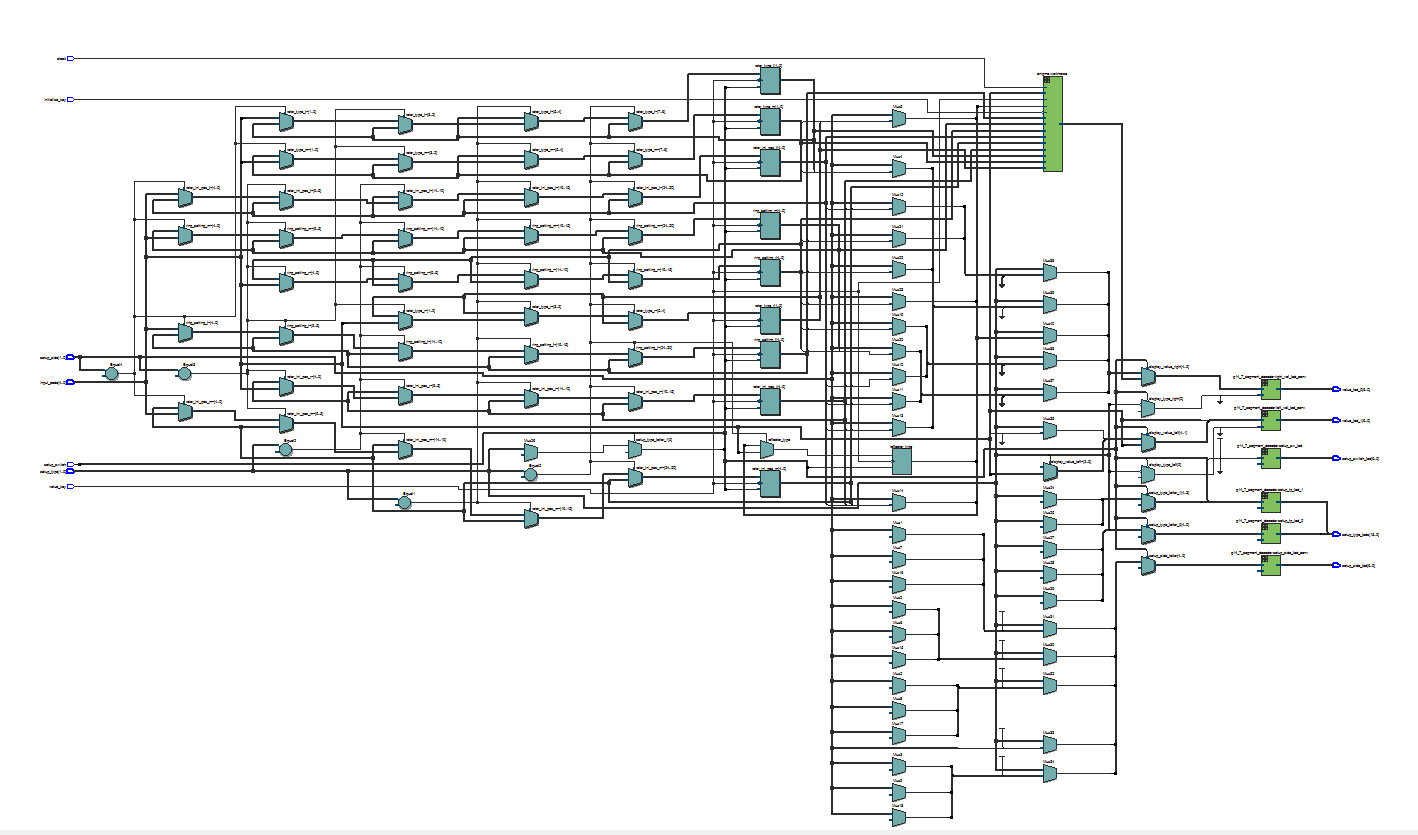
\includegraphics[scale=0.3]{interface_block_diag.PNG}
    \caption{Implementation of the Enigma's user interface hardware.}
    \label{fig:ui_block_diagram}
\end{figure}

\begin{figure}[ht!]
    \centering
    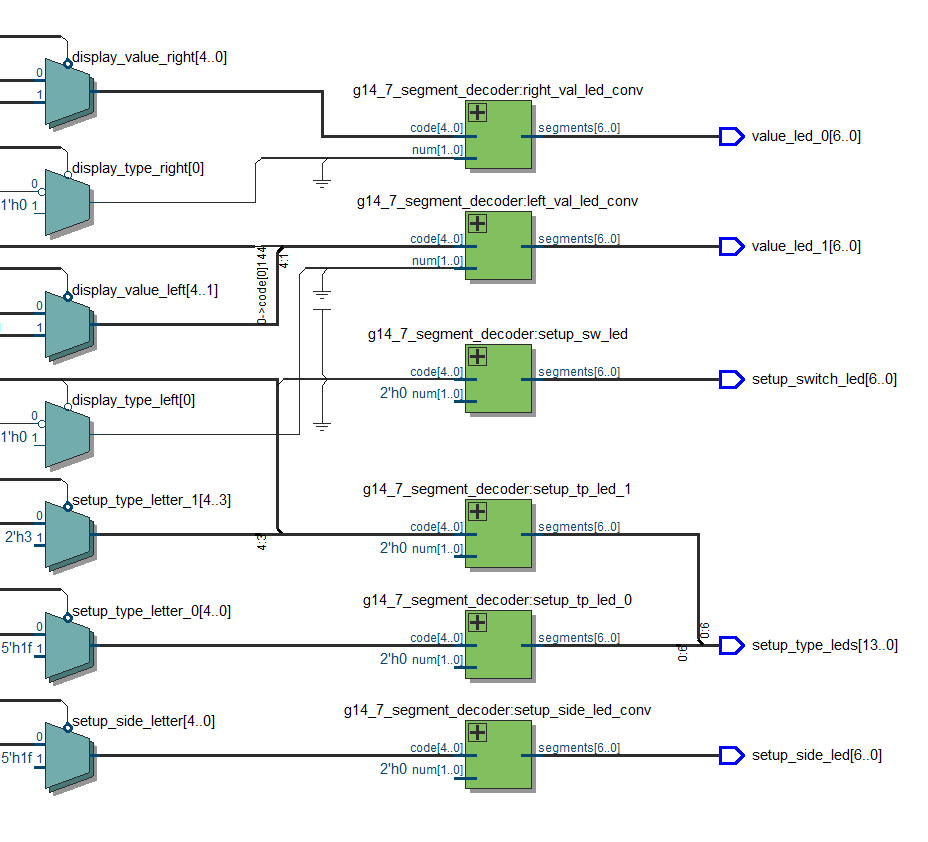
\includegraphics[scale=0.4]{seven_seg_decoders_block.PNG}
    \caption{Block of seven segment display decoders.}
    \label{fig:seven_segment_decoders}
\end{figure}

\begin{figure}[ht!]
    \centering
    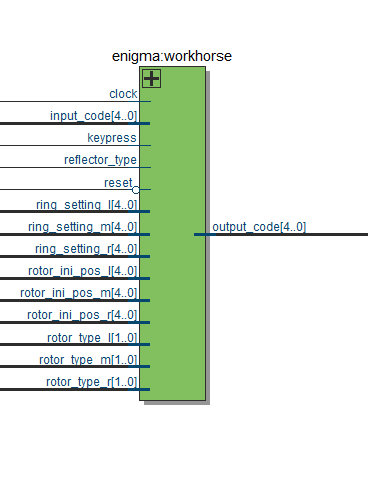
\includegraphics[scale=0.5]{enigma_block_diag.PNG}
    \caption{Block diagram of the actual Enigma scrambling mechanism.}
    \label{fig:enig_block_diag}
\end{figure}

\subsection{Enigma Implementation}
The actual Enigma machine is composed of several rotors as well as a finite state machine whose job it is to increment the appropriate rotors' rotor positions when key-press is asserted. There are other components within it, such as the stecker and the reflector, which we shall discuss shortly. 

\begin{figure}[ht!]
    \centering
    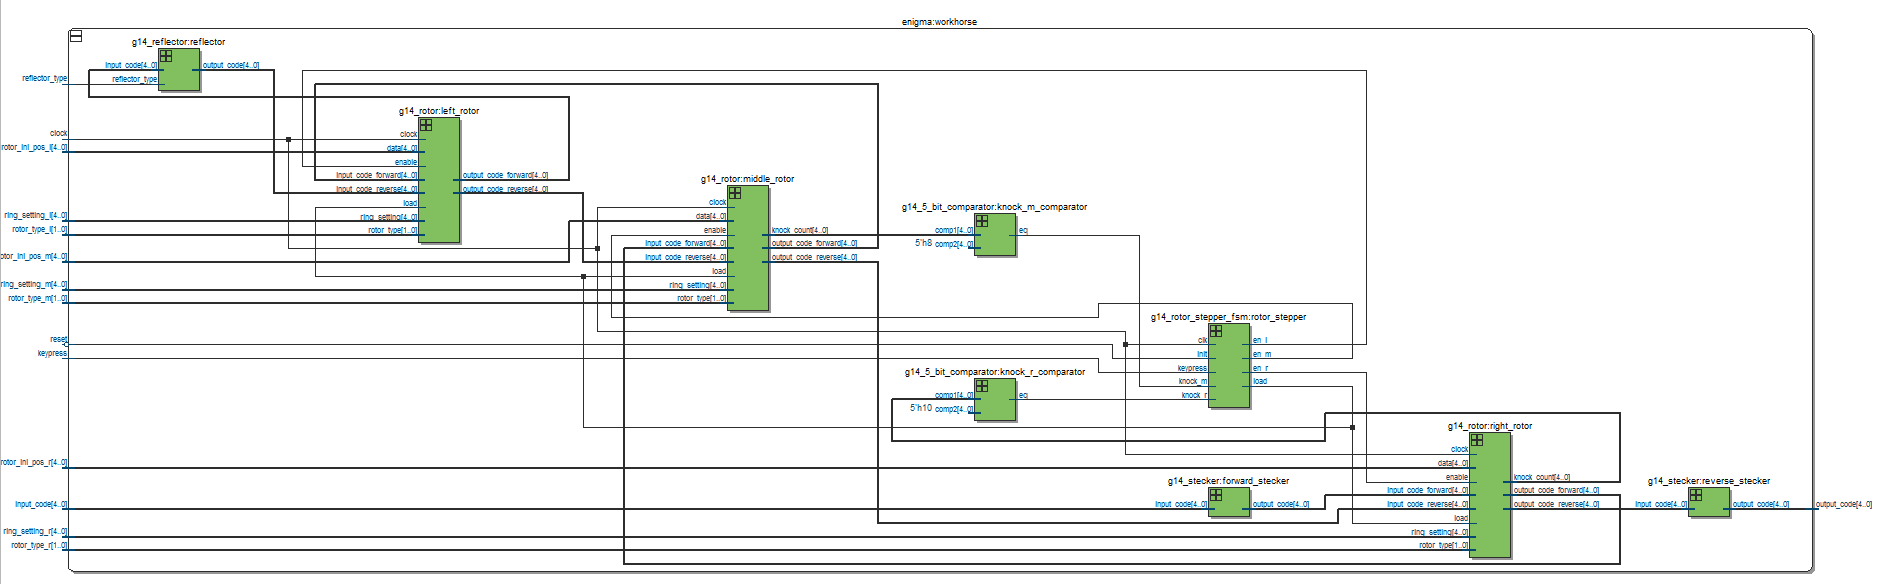
\includegraphics[scale=0.23]{enig_internal_block_diag.PNG}
    \caption{Complete internal block diagram of the Enigma scrambling mechanism. Refer to figures \ref{fig:enig_internal_block_diag_left} to \ref{fig:enig_internal_bl_diag_right} for a closer look at the components.}
    \label{fig:enig_internal_block_diag}
\end{figure}

\begin{figure}[ht!]
    \centering
    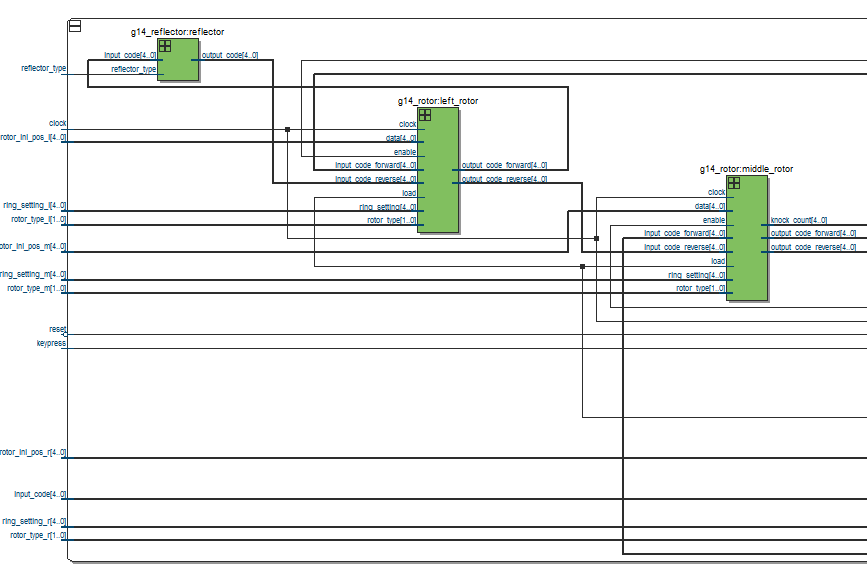
\includegraphics[scale=0.45]{enig_internal_left.PNG}
    \caption{A closer look at the components in the left side of the block diagram in figure \ref{fig:enig_internal_block_diag}.}
    \label{fig:enig_internal_block_diag_left}
\end{figure}


\begin{figure}[ht!]
    \centering
    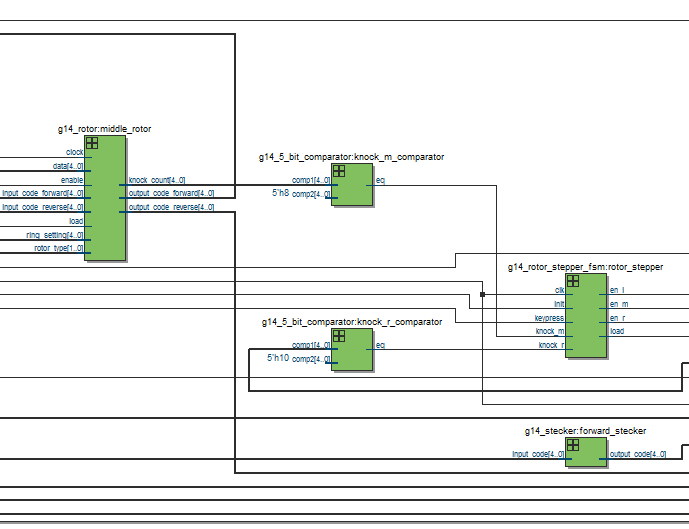
\includegraphics[scale=0.5]{enig_internal_middle.PNG}
    \caption{A closer look at the components making up the middle of the block diagram in figure \ref{fig:enig_internal_block_diag}.}
    \label{fig:enig_internal_bl_diag_mid}
\end{figure}

\begin{figure}[ht!]
    \centering
    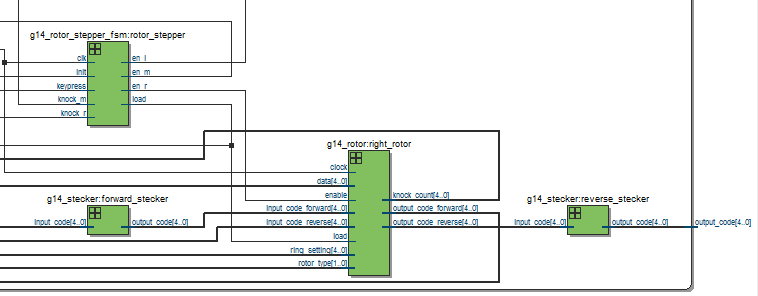
\includegraphics[scale=0.5]{enig_internal_right.PNG}
    \caption{A closer look at the components making up the right side of the block diagram in figure \ref{fig:enig_internal_block_diag}.}
    \label{fig:enig_internal_bl_diag_right}
\end{figure}

Let's first describe the general flow of two things, first the five bit wide \textit{input\_code} then the key-press bit. Each of these will be described in the following lists, with heavy references to figures \ref{fig:enig_internal_block_diag_left} through \ref{fig:enig_internal_bl_diag_right}. It is important that the reader sees how these diagrams fit into the overall system diagram of the Enigma in figure \ref{fig:enig_internal_block_diag} before proceeding. In our description of how the input progresses through the circuit, we will ignore the internal architecture and subtleties of the rotors, and simply refer to the outputs as being scrambled versions of the input. 
\begin{enumerate}
    \item The input code is sent to the input of the \textit{forward\_stecker} which can be seen in figure \ref{fig:enig_internal_bl_diag_right}. The stecker scrambles the input code and produces a temporary output\_code which can also be seen in figure \ref{fig:enig_internal_bl_diag_right}.
    \item The output of the stecker is connected to the \textit{input\_code\_forward} input of the right\_rotor which can be seen in figure \ref{fig:enig_internal_bl_diag_right}. Let's not concern ourselves just yet with how this rotor scrambles the input, but just know that it scrambles this forward input and the result is seen at \textit{output\_code\_forward}.
    \item This wire is connected to \textit{input\_code\_forward} of the middle\_rotor, which can be seen in figure \ref{fig:enig_internal_bl_diag_mid}. Again, let's simply consider that this input is scrambled and the output is set at \textit{output\_code\_forward}.
    \item This output code is in turn connected to \textit{input\_code\_forward} of the left\_rotor, which can be seen in figure \ref{fig:enig_internal_block_diag_left}. Again, the scrambled output is set to the \textit{output\_code\_forward}. 
    \item This signal is the input to the reflector, which can be seen in figure \ref{fig:enig_internal_block_diag_left}. The reflector consists of an invertible mapping of one letter to another, this means that if A as an input yields C as an output, then C as an input yields A as an output. The scrambled output is set at the output code. 
    \item From here we can follow the signal from the \textit{input\_code\_reversed} to the \textit{output\_code\_reversed} for the left\_rotor, then the middle\_rotor, and finaly the right\_rotor. 
    \item As a final scrambling step, the \textit{output\_code\_reversed} from the right\_rotor goes into the reverse\_stecker, which applies the inverse transformation of the original stecker on its input value, yielding the final result at its output. This reverse\_stecker can be seen in figure \ref{fig:enig_internal_bl_diag_right}.
\end{enumerate}

The next thing to understand is how the key-press impacts the Enigma functionality. From a high level, it rotates the rotor's positions, based on the knock values passed to the finite state machine, this changes the scrambling in a predictable manner if you know the correct starting configuration of the machine, and in an uncrackable way if you do not.  Before we can fully appreciate this, we need to understand the inner working of the rotors and the rotor stepper finite state machine. Let us elaborate the internal workings of these components so that we may truly grasp the impact of the key-press. 

\subsubsection{Stecker Circuit}
The stecker circuit scrambles the input and the reverse stecker scrambles it back the opposite way. Basically the stecker is a one-to-one mapping of the 26 possible inputs onto the 26 possible outputs. The inverse mapping is specified such that in the regular direction if A maps to B then in the inverse mapping B maps to A. Note that this does not say anything about what B maps to in the forward direction, nor what A maps to in the inverse direction. 

\subsubsection{Reflector Circuit}
The reflector circuit is similar to the stecker circuit in that it is a simple mapping. The difference is however that the mapping is invertible, that means an input of A yielding B means necessarily that an input of B would yield A.

\subsubsection{Knock Comparators}
These are simple five bit comparator circuits, which take two five bit wide inputs and assert the output if the two five bit words are identical. 

\subsubsection{Rotor Circuit}
The rotor circuit has a forward and reverse direction. The actual circuit is fairly linear, especially when compared to the Enigma machine. Figures \ref{fig:rotor_1} through \ref{fig:rotor_5} show the traversal of the rotor circuit. Let's again follow the input code through the circuit, explaining the various transformations that happen along the way. We will only consider the \textit{input\_code\_forward}, but the reverse path is pretty much exactly the same except for a difference in values on the shifting directions for some of the barrel shifters. The idea behind this difference in direction is that the input sequence is invertible: if you put a particular letter in in a particular rotor setting, then putting the result in as the input will yield the original input at the output. That being said, let's follow the \textit{input\_code\_forward} through the circuit. 
\begin{enumerate}
    \item The input code goes into the forward\_decoder\_0 which decodes the 5 bit input (interpreted as an unsigned) into the appropriate one hot encoded 26 bit binary representation. Ex: If the input code is `00110' (6), then the sixth least significant bit of the output 26 bit vector will be asserted. This can be seen in figure \ref{fig:rotor_1}.
    \item The now decoded signal goes into the forward\_barrel\_shifter\_0 where it is shifted to the right based on the current counter value. This can also be seen in figure \ref{fig:rotor_1}.
    \item The signal travels from the barrel shifter to another barrel shifter, which shifts the signal to the \textbf{left} based on the \textbf{ring settings} of the Enigma. This can be seen in figure \ref{fig:rotor_2}.
    \item The signal is now re-encoded back into its five bit representation by the forward\_encoder\_0 which can be seen in figure \ref{fig:rotor_2}.
    \item The signal is now sent to the forward\_permuter, which based on the rotor type for this particular rotor, maps each possible 5 bit input to a 5 bit output (both in the range of [0,25]). This can be seen in figure \ref{fig:rotor_3}.
    \item From the permuter the scrambled value is decoded once more, at the forward\_decoder\_1 (as seen in figure \ref{fig:rotor_3}).
    \item Now the signal passes on to the forward\_barrel\_shifter\_2 where it is shifted to the \textbf{right} based on the ring setting for this particular rotor (note that this is the opposite direction from before, and that the ring setting is shifting first. This is part of what makes the rotors invertible). This can be seen in figure \ref{fig:rotor_4}.
    \item The final scramble happens next, the signal is shifter \textbf{left} by the count (which we shifted the signal to the right by before). This can be seen in figures \ref{fig:rotor_4} and \ref{fig:rotor_5}.
    \item Finally, the 26 bit scrambled signal is encoded into a 5 bit vector and set at the output. 
\end{enumerate}


\begin{figure}[ht!]
    \centering
    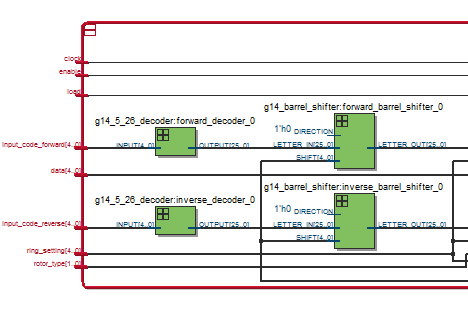
\includegraphics[scale=0.9]{rotor_1.PNG}
    \caption{The input ports and first layer of components of the rotor.}
    \label{fig:rotor_1}
\end{figure}

\begin{figure}[ht!]
    \centering
    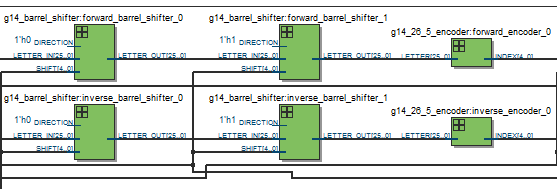
\includegraphics[scale=0.7]{rotor_2.PNG}
    \caption{The second layer of components of the rotor.}
    \label{fig:rotor_2}
\end{figure}

\begin{figure}[ht!]
    \centering
    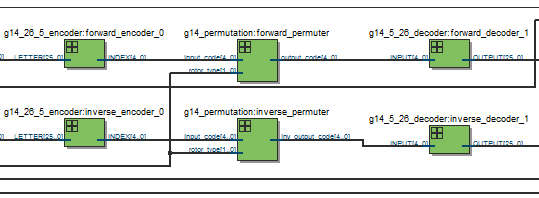
\includegraphics[scale=0.7]{rotor_3.PNG}
    \caption{The third layer of components of the rotor.}
    \label{fig:rotor_3}
\end{figure}

\begin{figure}[ht!]
    \centering
    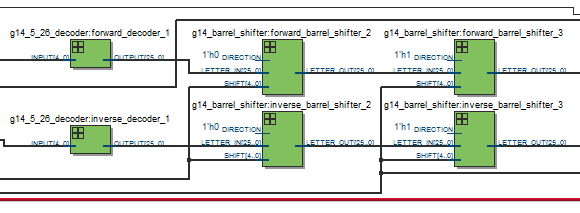
\includegraphics[scale=0.6]{rotor_4.PNG}
    \caption{The fourth layer of components of the rotor.}
    \label{fig:rotor_4}
\end{figure}

\begin{figure}[ht!]
    \centering
    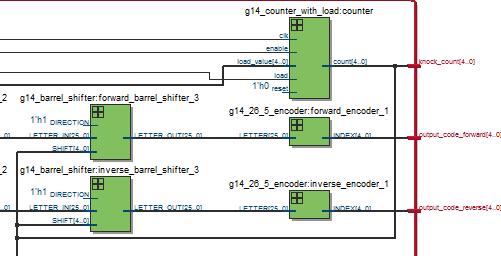
\includegraphics[scale=0.7]{rotor_5.PNG}
    \caption{The final layer and output ports of the rotor. }
    \label{fig:rotor_5}
\end{figure}


\subsubsection{Rotor Stepper FSM}
In the rotor circuit, we mentioned a count value which we shifted by in the first and last barrel shifter. These count values are incremented based on the Rotor Stepper FSM. The Finite State machine has 8 possible states. The block diagram of the Rotor Stepper FSM can be seen in figure \ref{fig:fsm_block_diag}. Overall, there are only two things you need to know about the rotor stepper FSM: 
\begin{enumerate}
    \item Pressing the init button puts the FSM in state 0 where it asserts the load signal which tells all of the rotors to reset their current rotor positions (i.e. the count value we saw before) to the one specified in the settings (i.e. held in the register in the user interface level circuitry). 
    \item Pressing and releasing the action button shifts the FSM through states 2 and 3, and depending on the current count and whether it is a notch in the rotor, it enables the appropriate counter increments. 
\end{enumerate}
In effect this is the driver of the count values that we use to shift within each of the rotors. 

\begin{figure}
    \centering
    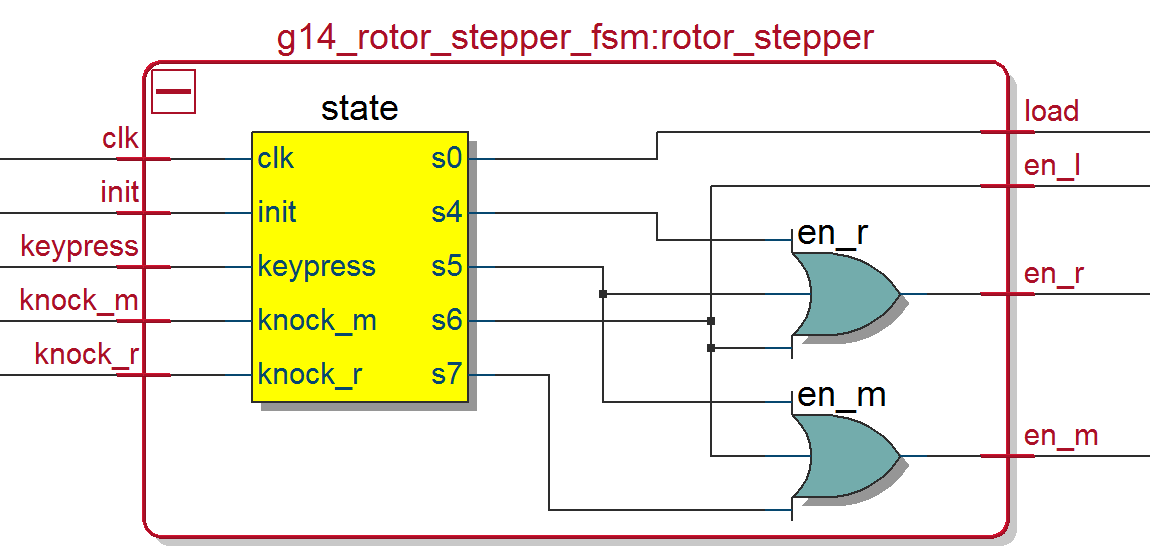
\includegraphics[scale=0.3]{fsm_block_diag.PNG}
    \caption{High level block diagram of the finite state machine.}
    \label{fig:fsm_block_diag}
\end{figure}

\subsection{Final Remarks}
We now understand the way the Enigma functions internally. Apart from the initial settings, the only things that is dynamic in the scrambling is the count values which are incremented based on the FSM and triggered by the KeyPress signal. The preceding sections have been fairly involved, describing the implementation behind the functionality. For a better understanding of how to actually use the Enigma, refer to the following section.


\section{Interface Guide} \label{guide}

\subsection{Labels \& Shorthand}
Before we get started, it is useful to describe some shorthand notation for displays and switches on the board. You can see the slides switches and their corresponding annotations in figure \ref{fig:slide_switch_shorthand}. The seven segment LED displays are labeled, from left to right, HEX5 down to HEX0, which you can see on the board. The push buttons are labeled from left to right KEY3 down to KEY0, which can also be seen on the board. From here on out I will refer to everything by its shorthand name. 

\begin{figure}[ht!]
    \centering
    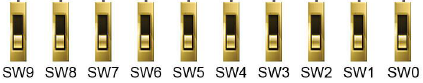
\includegraphics{slide_switch_shorthand.PNG}
    \caption{Display of the slide switches and their appropriate labels \cite{soc_manual}.}
    \label{fig:slide_switch_shorthand}
\end{figure}

\subsection{Buttons}
There are two buttons which impact the functionality of the board. KEY3 is the \textbf{action button}. It is the button you hit to set values, and will be referred to as the \textit{action button} from now on. KEY0 is the \textbf{reset button}. While encoding or decoding values using the Enigma machine, you can reset the rotors to the daily settings by hitting this button. More details on this will become clear in the following sections. This button will be referred to as the \textit{reset button} from now on. 

The two buttons were placed far apart to avoid accidentally hitting the wrong button. Accidentally depressing the reset button would require the user to restart the message encoding / decoding procedure entirely, which is not something that we want to have happen. 

\subsection{Operation Mode} \label{oppmode}
Let's briefly ignore the various setup tools made available to us and use the default settings to get a good idea of how the operation of the Enigma works. In order to get into operation mode, all you need to do is make sure that \textbf{SW9} (or the \textit{setup\_switch}) is down. You will know you are in operation mode if \textbf{HEX5} (the left most display) is displaying the letter O. 

\subsubsection{Operation Displays}
In operation mode \textbf{HEX1} indicates the current letter that you have selected by your input switches (refer to table \ref{tab:gen_switch_func} for indication of what these switches are). \textbf{HEX0} indicates the current translation of your input value by the Enigma machine. \textbf{The general procedure for encoding a message is the following: }
\begin{itemize}
    \item Push and release the reset button.
    \item Set the input switches to the value you want to input, which you can verify in \textbf{HEX1}.
    \item Push and release the action button. You will notice that HEX0 will change when you press the action button. Note that it does not necessarily need to change though. 
    \item The encoded letter for your input is the letter in HEX0. Write down HEX0. 
    \item Repeat steps 2 through 5 until you have completed your message. 
\end{itemize}


\textbf{Likewise the decoding procedure is as following: }

\begin{itemize}
    \item Push and release the reset button.
    \item Set the input switches to the value you want to decode, which you can verify in \textbf{HEX1}.
    \item Push and release the action button. You will notice that HEX0 will change when you press the action button. Once again, it doesn't necessarily need to change. 
    \item The decoded letter for your input is the letter in HEX0. Write down HEX0. 
    \item Repeat steps 2 through 5 until you have completed decoding your message. 
\end{itemize}

Note that the above procedure assumes that the Enigma you are encoding and decoding with are set to the same \textit{initial settings}. We will discuss initial settings later in this guide. 

This is all you need to know as far as the general operation of the Enigma is concerned. However, the most important part of the Enigma machine's encryption is being able to change the initial setting of the machine. The setup of the machine is discussed in the following sections. 

\subsection{Switches} \label{switches}
Before we can dive into the different setup configurations of the Enigma, it is important to understand the switches and their general purpose. There are nine switches on the FPGA, all of which are used to some extent for the user interface of the Enigma. They are broken up into four distinct groups as you can see in table \ref{tab:gen_switch_func}. Each of the groups' options and particularities are explained in the appropriate section. 

\begin{table}[ht!]
    \centering
    \begin{tabular}{|c|c|c|}
        \hline
        Group & Switches & Functionality \\
        \hline \hline
        Setup& \small{SW9} & \footnotesize{Toggles between setup and operation mode} \\
        \hline
        Setup Type & \small{SW8 \& SW7} & \footnotesize{Allows us to select what we are setting up (4 options)} \\
        \hline
        Setup Side & \small{SW6 \& SW5} & \footnotesize{Allows us to select which side we are setting up} \\
        \hline
        Input Value & \small{SW4-SW0} & \footnotesize{Allows us to input values between 0 and 31} \\
        \hline
    \end{tabular}
    \caption{Description of the switches on the board and their functionality.}
    \label{tab:gen_switch_func}
\end{table}

\subsection{Configuration} \label{config}
There are four different settings of the Enigma, each of which have multiple possible options. The following section explains each of these settings and their possible values, as well as how to set them up. First thing is first, to get into setup mode, put the setup switch high (SW9). Tables \ref{tab:setup_types} and \ref{tab:setup_sides} show how the slide switches impact which setup mode we are in, and the following sections describe how to use this to effectively set up the Enigma machine.


\begin{table}[ht!]
    \centering
    \begin{tabular}{|c|c|c|c|}
        \hline
        Setup Type & SW8 & SW7 & Displays \\
        \hline \hline
        Reflector & 0 & 0 & RF \\
        \hline
        Rotor Type & 0 & 1 & RT \\
        \hline 
        Rotor Initial Positions & 1 & 0 & IP \\
        \hline
        Ring Setting & 1 & 1 & RS \\
        \hline
    \end{tabular}
    \caption{Setup types and their switch configurations.}
    \label{tab:setup_types}
\end{table}


\begin{table}[ht!]
    \centering
    \begin{tabular}{|c|c|c|c|}
        \hline
        Setup Side & SW6 & SW5 & Displays \\ 
        \hline \hline
        Right & 0 & 0 & R \\
        \hline
        Middle & 0 & 1 & M \\
        \hline
        Left & 1 & D & L \\
        \hline
    \end{tabular}
    \caption{Setup sides and their switch configurations.}
    \label{tab:setup_sides}
\end{table}

\subsubsection{Reflector}
In the chain of scrambling of the Enigma, the reflector scrambles the forward going path and send it back on its way down the reverse path. From the users perspective there are two possible values that the reflector can be set to (i.e. two mappings from the forward output to the reverse input). In order to set the reflector, you need to have both of the \textit{setup type} switches down (SW8 and SW7). You will know you are setting up the correct setting if HEX3 and HEX2 read `RF'. In this state, you can see the current value of the reflector (0 or 1) in HEX0. You can use SW0 to choose a value for the reflector (which you can verify in HEX1) and you can set the reflector value by pushing the action button. 

\subsubsection{Rotor Type}
Each rotor (there are three) has a mapping from one letter to another (or in some cases itself). These mappings are what scramble the input code. There are four different possible mappings for each rotor of this particular Enigma machine. In order to set a particular rotor's type, we must get into the `rotor type' setup mode, and we must select the appropriate rotor (right, middle, left) at which point we can set the particular value. 

Refer to table \ref{tab:setup_types} in order to see where to set switches 7 and 8 to get into \textit{Rotor Type} mode. From there you can pick which side you want to set using switches 5 and 6 (consult table \ref{tab:setup_sides} to see how to pick a particular side). Once you have picked a side, HEX0 will show the current rotor type of that side. You can adjust the value sliders (SW4-SW0) to pick a rotor type value between 1 and 4. The current value being interpreted based on your inputs is displayed in HEX1. Set the value to what you want and press the action button to set the rotor type to the value you have selected. 


\subsubsection{Rotor Initial Positions}
If each rotor started at the same point every time we encrypted a message, the encryption wouldn't be very difficult to crack at all. Luckily for us, we are able to start each of the three rotors at any of 26 initial positions, we can even change them on the fly using agreed upon techniques if both the person encoding the message and the person decoding the message know how to follow along. 

Again refer to table \ref{tab:setup_types} in order to see where to set switches 7 and 8 to get into \textit{Rotor Initial Positions} mode. From there you can once again pick which side you want to set using switches 5 and 6. HEX0 will show the current starting letter (initial position) of the particular rotor and HEX1 will display the currently selected value of the input slide switches (SW4-SW0). Once you have picked the value that you would like, you may press the action button and you will set the rotor initial position. 

\subsubsection{Ring Setting}
On top of the initial positions of the rotors, we have an initial scrambling step called the ring setting. There is a particular ring setting for each of the three rotors and each ring setting can be set independently. 

Once again, refer to table \ref{tab:setup_types} in order to see where to set switches 7 and 8 to get into \textit{Ring Setting} mode. From there you can once again pick which side you want to set using switches 5 and 6. HEX0 will show the current ring setting (a letter between A - Z symbolizing the shift) of the particular rotor and HEX1 will display the currently selected value of the input slide switches (SW4-SW0). Once you have picked the value that you would like, you may press the action button and you will set the ring setting for the particular rotor.


% TODO include simulation stuff
\section{Testing}
The system was tested in simulation for each of its components. Most of these components have been shown in previous lab reports, so we will focus on two new components as well as the overall system testing. 
\subsection{Stecker}
The stecker circuit scrambles the inputs of the Enigma machine. It provides a one to one mapping from the 26 possible inputs to the 26 possible outputs. You may see the results of all 26 inputs being applied to the stecker circuit in figure \ref{fig:stecker_sim}. 


\begin{figure}[ht!]
    \centering
    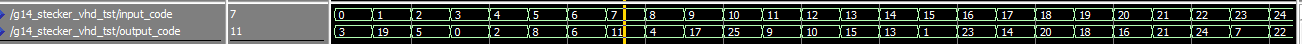
\includegraphics[scale=0.35]{stecker_sim.PNG}
    \caption{Simulation for all possible 26 inputs to the stecker with outputs displayed. }
    \label{fig:stecker_sim}
\end{figure}


\subsection{Reflector}
The reflector provides an invertible scrambling step to the input. This means that if an input A yields B then an input of B must yield A. You may see the simulation results of these simulations in figures \ref{fig:reflectorB} and \ref{fig:reflectorC}.


\begin{figure}[ht!]
    \centering
    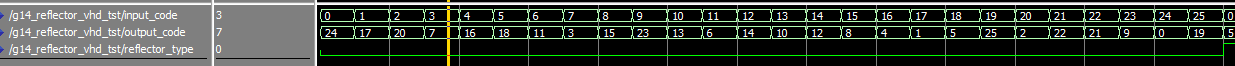
\includegraphics[scale=0.35]{reflectorB.PNG}
    \caption{The reflector circuit being tested in its \textbf{B} setup.}
    \label{fig:reflectorB}
\end{figure}


\begin{figure}[ht!]
    \centering
    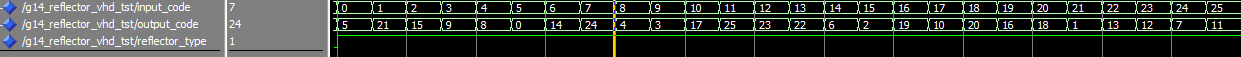
\includegraphics[scale=0.35]{reflectorC.PNG}
    \caption{The reflector circuit being tested in its \textbf{C} setup.}
    \label{fig:reflectorC}
\end{figure}

\subsection{Enigma Simulation}
The overall simulation results of the Enigma machine are shown in two separate cases in figures \ref{fig:enig_sim1} and \ref{fig:enig_sim2}. As you can see figure \ref{fig:enig_sim1} we input a sequence of values who upon keypress yield 0 at the output. Then we reset the Enigma, and input 0, at which point the original input sequence arises at the output. We do the same thing for the setup in figure \ref{fig:enig_sim2}, the difference is that we have a different internal setup for the Enigma machine. 

\begin{figure}[ht!]
    \centering
    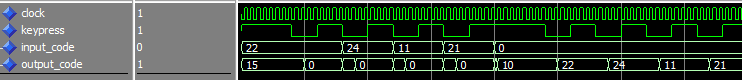
\includegraphics[scale=0.35]{enigma_sim_1.PNG}
    \caption{The Enigma simulation with setup \textbf{a}.}
    \label{fig:enig_sim1}
\end{figure}


\begin{figure}[ht!]
    \centering
    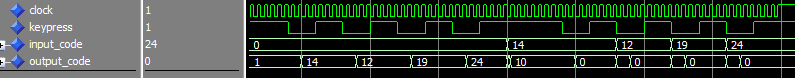
\includegraphics[scale=0.35]{enigma_sim_2.PNG}
    \caption{The Enigma simulation with setup \textbf{b}.}
    \label{fig:enig_sim2}
\end{figure}


\subsection{Full System Testing}
The system was tested by using multiple setups and attempting to encode and decode messages using the Enigma. 

\section{Resources \& Timing}
The system uses a total of 60 registers. These memory elements are comprised of the memory elements required to hold the current setting in the user interface, the current count in the counter mechanisms, and the state machine's state. The design uses 55 (12\%) of the pins available on the board, which is not really of much concern as it is not constrained in any way. It uses 2,456 of 32,070 available ALMs in terms of actual combinational logic (which comes out to about 8\% of the available logic units on the board). This comes down to the fairly complex user interface logic. The user interface could have been made much more simple in hardware, but it would have been at the loss of ease of use from the end user's perspective. Since the point of the user interface was to be easy to use, and not necessarily the most hardware efficient, this is acceptable. The other combinational logic is happening everywhere inside the rotors appart from the counters. 

The slow model's $F_{max}$ was found to be 88.28 MHz based on the hardware implementation. There were no constraints placed on the clock of the board in this analysis, so a discussion of slack and hold times does not add to our understanding of the timing of the circuit. However, from the slow model's $F_{max}$ we can see that it will in fact meet the timing constraints of the board. The frequency of the clock on the board is 50MHz, and since the $F_{max}$ of our circuit is significantly higher than this, we do not need to worry about errors in the sequential logic.

\section{Conclusion}
Now that we have discussed how the system works and how it was tested, let us briefly discuss some of the difficuties and potential enhancements for the Enigma. 

\subsection{Issues}
The only major issue which blocked progress and impacted development was the fact that the 5 to 26 decoder was in fact faulty. Originally we wrote the decoder behaviorally with a simple for loop, however we were required to re-implement the decoder using a structural approach (select statements). In doing so we introduced a bug (obviously, since the structural code is unclear and close to 30 lines longer, with each line containing at least 4 or 5 more operations than any given line in the loop). This decoder did not impact anything until the final machine was assembled, at which point it took some serious debugging to find the issue. In the end, we re-wrote the decoder behaviorally in order to avoid the complexity of the structural approach. 

\subsection{Enhancements}
There is a lot of room for enhancement on the Enigma. The easiest way for me to elaborate is to simply provide a list of potential enhancements: 
\begin{itemize}
    \item The ability to rotate the rotors back by one if you make a mistake, this prevents you from needing to reset and restart the encoding of the entire message if you make a mistake. 
    \item The ability to see how many characters you have so far encrypted, this allows you to know the current length of your word, which is a way of checking if you are where you expect to be. 
    \item Expanding on the previous idea, the ability to simply see the entire input message and the entire output message side by side would be extremely helpful. Along with this we would require a better display and a more elaborate value-in mechanism. 
    \item Include a few syntax characters in the remaining configurations of the 5 bit word. Notably we could include a space, a comma, a period, and potentially others. 
\end{itemize}
\clearpage

\bibliographystyle{unsrt}
\bibliography{bibliography}

\end{document}
